\documentclass[11pt,a4paper,onecolumn,oneside]{tau-class/tau}
\usepackage{fontspec}
\setmainfont{TeX Gyre Termes}
\usepackage{unicode-math}
\setmathfont{TeX Gyre Termes Math}
\usepackage[english]{babel}
\usepackage{tabularx}
\geometry{margin=22mm,bottom=25mm}
\setlength{\emergencystretch}{2em}
\raggedbottom
\setcounter{topnumber}{2}
\setcounter{bottomnumber}{2}
\setcounter{totalnumber}{4}
\renewcommand{\topfraction}{.85}
\renewcommand{\bottomfraction}{.7}
\renewcommand{\textfraction}{.12}
\renewcommand{\floatpagefraction}{.75}
\definecolor{taucolor}{HTML}{245D4B}
\hypersetup{pdftitle={Price, nutrition and environmental performance within food categories},pdfauthor={Food Prices, Nutrition and Environmental Impact project}}
\doctype{Course research report}
\title{Price, nutrition and environmental performance within food categories}
\author{Food Prices, Nutrition and Environmental Impact project}
\dates{11 November 2026 | France | R for Data Science}
\footinfo{Food comparison}
\organization{Course research}
\leadauthor{France / 2024--2025 prices}
\theday{11 November 2026}
\renewcommand{\abstractname}{Abstract}
\AtBeginDocument{\renewcommand{\abstractname}{Abstract}}
\begin{abstract}
How do higher prices relate to nutritional and environmental performance within a food category? We link French Open Prices observations from 2024--2025 with Open Food Facts information retrieved in 2026 and conduct within-category exploratory analysis of 598 products in four categories. Cereals and dark chocolate show favourable price associations with both composite scores, while biscuits and juices show near-zero associations. Higher-priced chocolate combines lower sugar with higher saturated fat. Of 583 products with price and both grades, 562 have a cheaper same-category candidate with neither grade worse. The findings support setting a unit-price budget within a category and then comparing grades and composition. A bilingual Shiny dashboard supports chart exploration and two-product comparison.
\end{abstract}
\keywords{consumer choice, unit price, nutrition, environmental grades, Shiny}
\begin{document}
\maketitle\thispagestyle{firststyle}
\section{Introduction}
Consumers comparing two packaged foods must consider price, nutrition and environmental performance together. Pack sizes differ, so the shelf price alone leaves part of the comparison unresolved. After converting both products to a price per kilogram or litre, a further question remains. Do higher-priced products within the same food category tend to have better nutritional and environmental profiles? Retail product analysts face a related question when assessing the attributes associated with a premium price.

Previous research shows that these relationships depend on the scale of comparison. Using 100 g or 100 kcal as the functional unit can change the relationships between food prices and sustainability measures\cite{masset2015}. International evidence also identifies differences between food groups in their price--attribute relationships\cite{martinez2025}. Product-level work supports examining nutrition and environmental performance together\cite{clark2022}. These findings motivate within-category analysis with both composite scores and individual nutrient quantities.

We study biscuits, breakfast cereals, dark chocolate and fruit juices with recorded prices in France. \textbf{RQ1} asks how unit price relates to nutritional scores and composition within each category. \textbf{RQ2} asks how unit price relates to environmental scores. \textbf{RQ3} asks which products have a lower-priced same-category alternative with neither grade worse. The first two questions describe patterns across products. The third translates those patterns into individual comparisons.

\section{Data and Methods}
\subsection{Sources and sample}
Open Prices provides euro-denominated observations for barcoded products in French stores in 2024--2025. Open Food Facts supplies product information retrieved on 2 November 2026, including pack size, nutrients and scores. Character barcodes link the two sources. The unit of comparison is one distinct product barcode.

Among 3,002 candidates meeting category, quantity and regular-price criteria, we sampled 150 products from each category with the fixed seed 20261102. Quantity conflicts or missing quantities excluded two products, leaving 598 products and 1,541 linked price observations. Selection retained products with missing scores. Each analysis then uses the fields required for its question. Equal category samples support comparison of within-category patterns.
\begin{table}[!ht]\centering\small\caption{Product counts, category median prices and grade coverage. Each product receives equal weight in the category summaries.}\begin{tabular}{lrlrrr}
\toprule
Category & $n$ & Unit & Median & Nutrition $n$ & Environment $n$ \\
\midrule
Biscuits & 149 & EUR/kg & 11.09 & 147 & 148 \\
Breakfast cereals & 150 & EUR/kg & 8.27 & 147 & 150 \\
Dark chocolate & 149 & EUR/kg & 25.83 & 146 & 149 \\
Fruit juices & 150 & EUR/L & 2.85 & 145 & 149 \\
\bottomrule
\end{tabular}
\label{tab:sample}\end{table}

\subsection{Price, nutrition and environmental measures}
Biscuits, cereals and chocolate use EUR/kg, and juices use EUR/L. A product's representative price is the median of its valid non-discounted unit offers after duplicate-combination handling. Offer counts and dates remain available in the product comparison.

Nutrition uses Nutri-Score 2023, with grades A--E and lower numerical scores indicating better profiles. Sugar, saturated fat and fibre are expressed per 100 g, or per 100 ml for juices. Environmental grades run from A+ to F, with higher numerical scores indicating better performance. During validation we found 16 valid F grades classified as missing by an earlier cleaning rule. We restored them from the saved product responses and paired them with French scores. Environmental grades then covered 596 products, and 583 products had price and both grades.

\subsection{Exploratory analysis}
We examined field coverage and unit-price distributions, compared prices across grades with boxplots, and calculated Spearman rank correlations within categories. The coefficient $\rho$ describes the direction and degree of association between rankings of price and an attribute. Each coefficient uses products with both numerical values available and is reported with its own sample size. Price-distribution figures use logarithmic axes to display wide ranges clearly.

For RQ3, we searched within each category for a product with a strictly lower representative price and nutrition and environmental grades each at least as good. Each grade scale retains its own order. Recipe and pack details remain part of the subsequent comparison of suitability.

Sensitivity analyses use discounted offers, retained duplicate observations, annual prices and price per 100 kcal, and separately inspect products with at least two regular offers. Alternative price definitions are compared with the main definition on the same products. AGRIBALYSE 3.2 carbon estimates are aggregated by standard reference food and retain their kg CO$_2$e/kg food unit.

\section{Results}
\subsection{Price--score relationships vary by food category}
Higher prices in breakfast cereals and dark chocolate tend to accompany lower nutrition scores and higher environmental scores. Both associations are close to zero for biscuits and juices. Table~\ref{tab:associations} answers RQ1 and RQ2 by showing this variation across the four categories.
\begin{table}[!ht]\centering\scriptsize\caption{Within-category Spearman correlations between price and composite scores. Lower nutrition scores and higher environmental scores indicate better profiles. Each coefficient uses its own complete sample.}\begin{tabular}{lrrrr}
\toprule
Category & Nutrition $n$ & $\rho$ price--nutrition & Environment $n$ & $\rho$ price--environment \\
\midrule
Biscuits & 147 & 0.022 & 148 & 0.030 \\
Breakfast cereals & 147 & -0.196 & 150 & 0.307 \\
Dark chocolate & 146 & -0.271 & 149 & 0.243 \\
Fruit juices & 145 & 0.025 & 149 & 0.035 \\
\bottomrule
\end{tabular}
\label{tab:associations}\end{table}

\begin{figure}[!htbp]\centering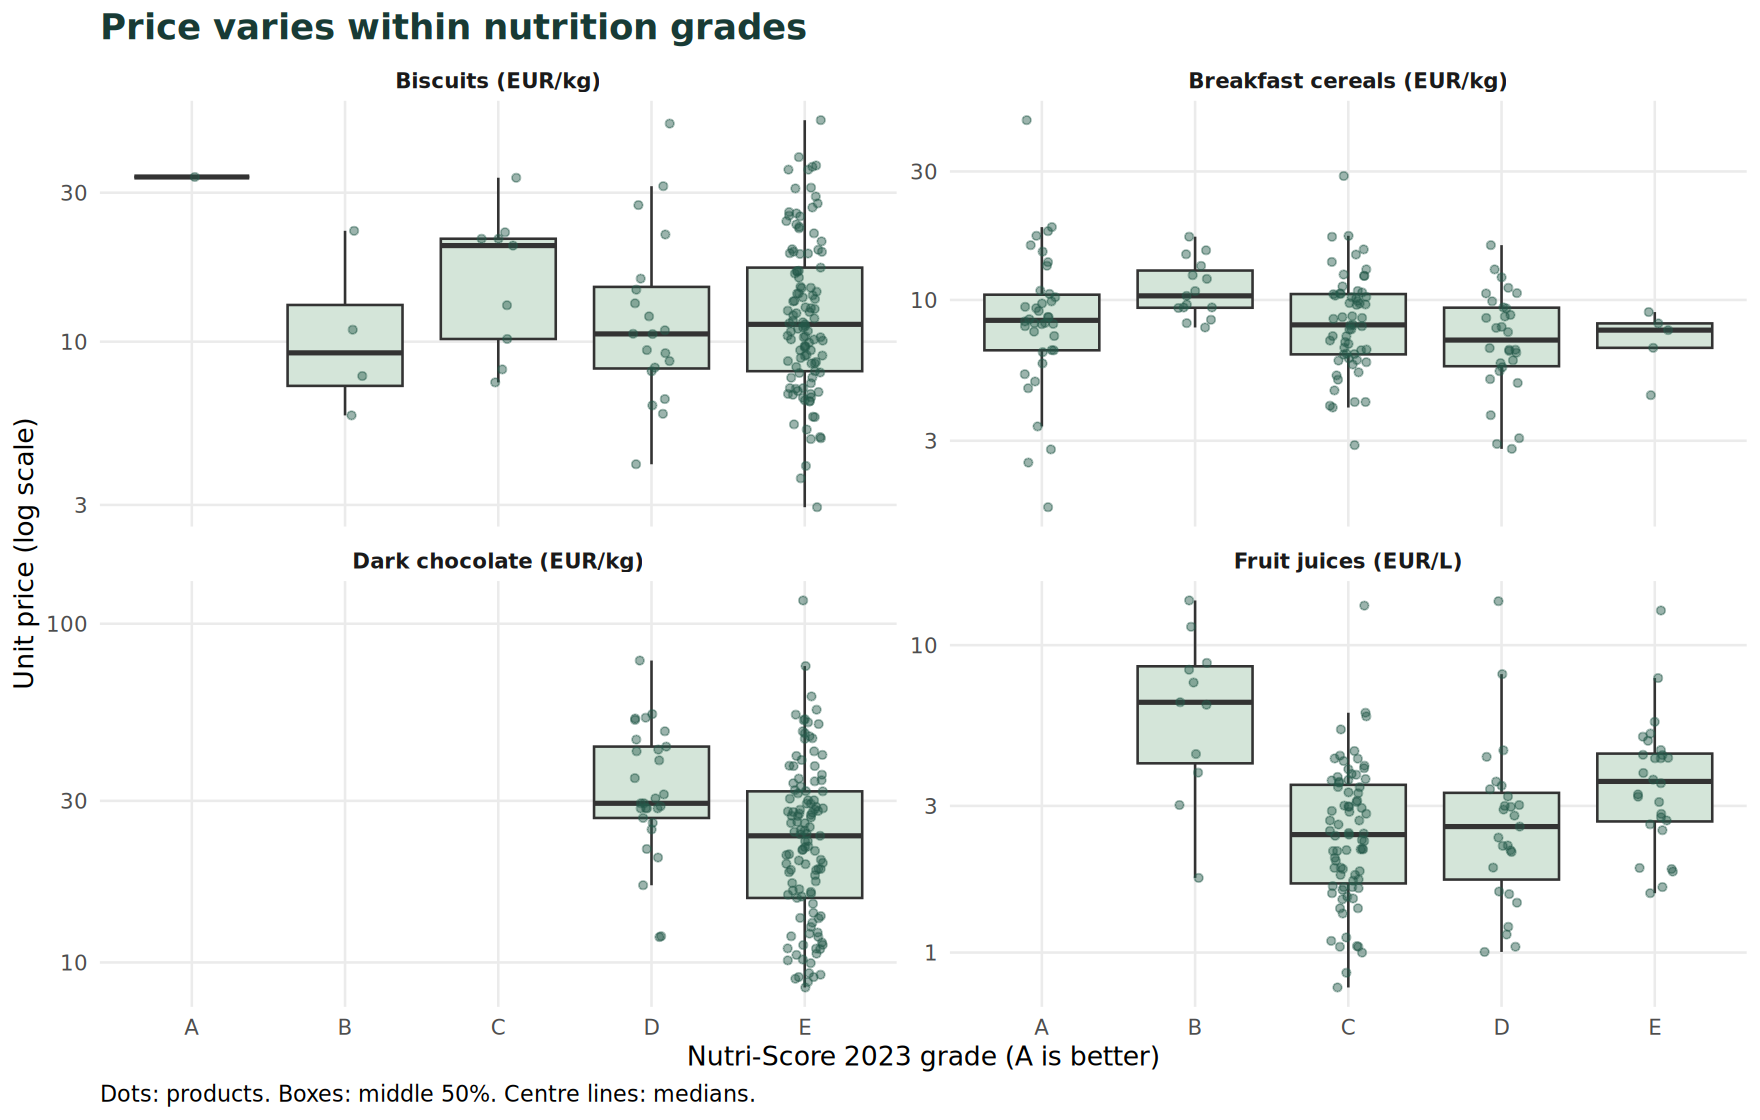
\includegraphics[width=\linewidth,height=.32\textheight,keepaspectratio]{generated/figures/en/price_nutrition.png}\caption{Products within the same nutrition grade still differ in price. The horizontal axis shows Nutri-Score grades and the vertical axis shows logarithmic unit price. Each dot is a product. Boxes contain the middle 50\% of prices and centre lines show medians. Category panels have independent price scales.}\label{fig:nutrition}\end{figure}

Figure~\ref{fig:nutrition} adds distributional detail to the correlations. Of 147 biscuits with nutrition grades, 113 have grade E and only one has grade A. Dark chocolate has only grades D and E. Individual nutrient quantities therefore provide additional information for comparing products within these concentrated grade groups.

\begin{figure}[!htbp]\centering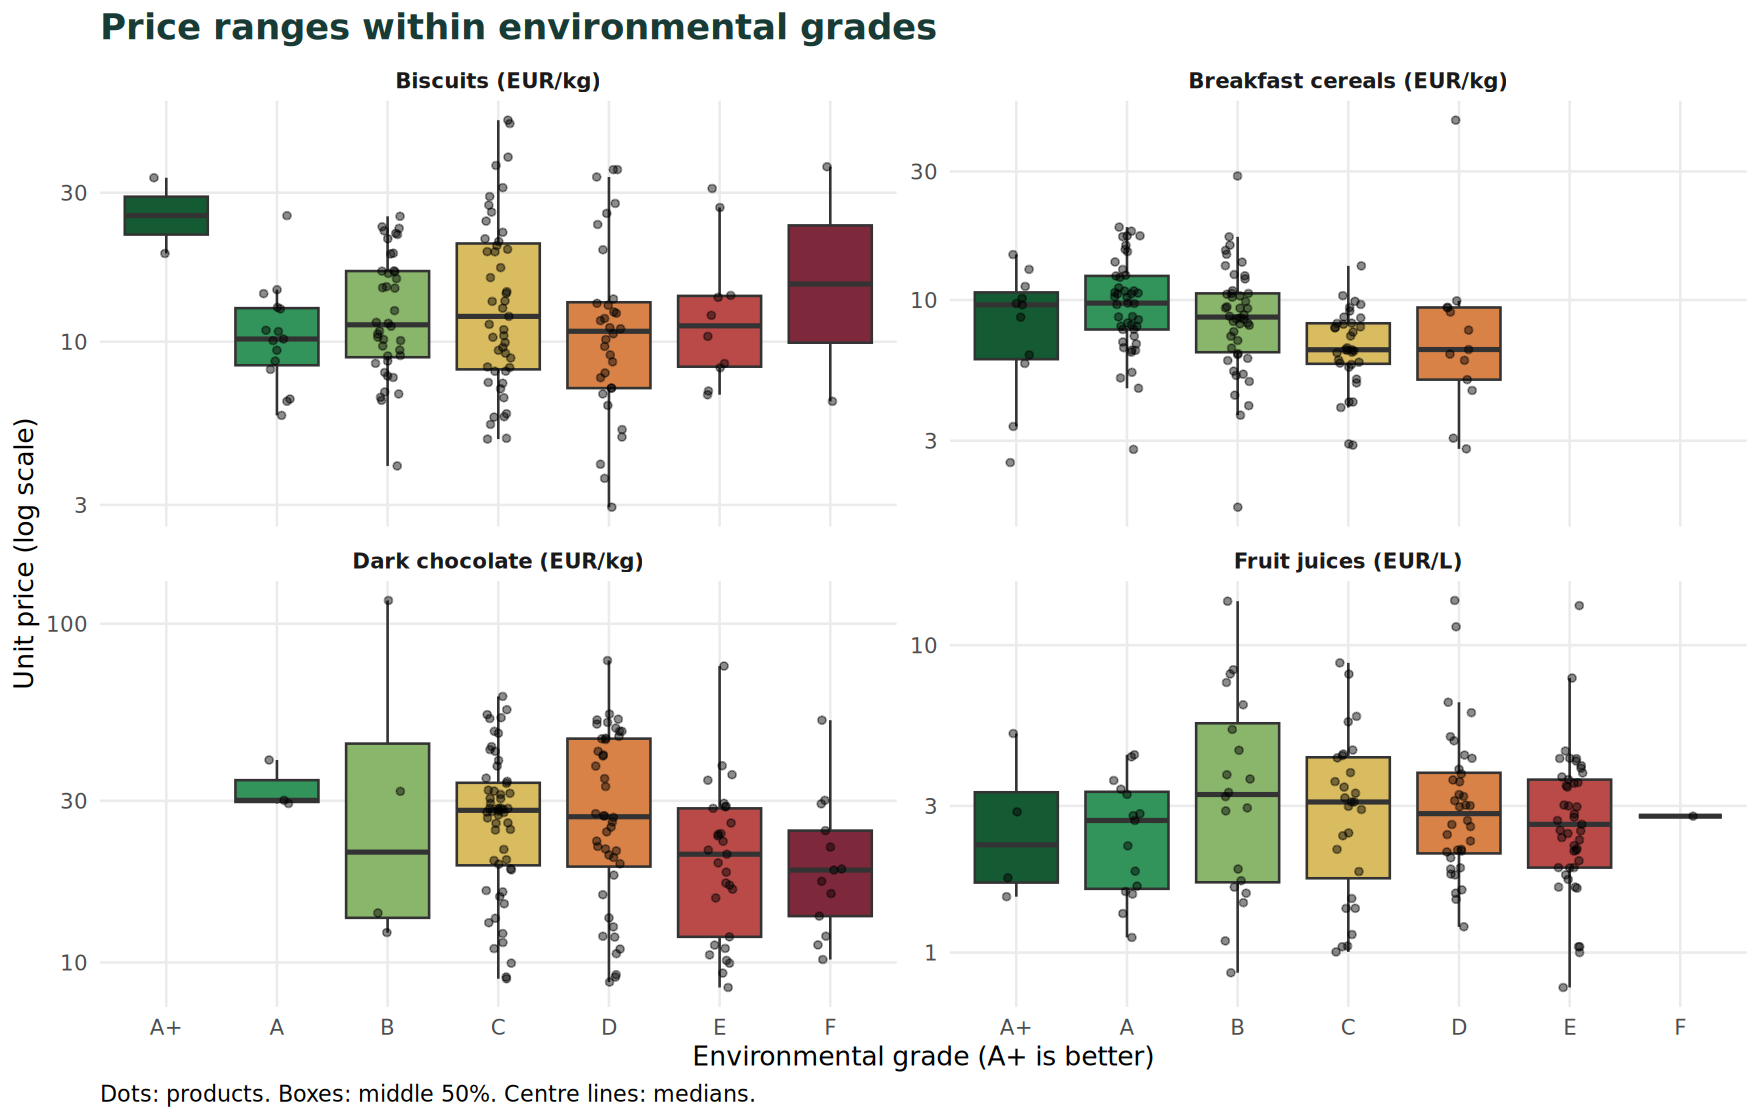
\includegraphics[width=\linewidth,height=.32\textheight,keepaspectratio]{generated/figures/en/price_environment.png}\caption{Historical unit prices by environmental grade. The horizontal axis runs from A+ to F and the vertical axis shows logarithmic unit price. Each dot is a product, with boxes and centre lines showing the middle 50\% and median. Correlations in Table~\ref{tab:associations} use the corresponding numerical environmental scores.}\label{fig:environment}\end{figure}

Price--environment correlations are $\rho=0.307$ for cereals and $0.243$ for dark chocolate. These categories show some association between higher prices and better environmental scores. The coefficients are $0.030$ for biscuits and $0.035$ for juices. Figure~\ref{fig:environment} shows the price ranges within grades, allowing further comparison among products at the same grade.

\subsection{Dark chocolate shows a sugar--saturated-fat trade-off}
Across 148 chocolates with sugar quantities, price and sugar have $\rho=-0.456$. Across 148 with saturated-fat quantities, the coefficient is $\rho=0.401$. Higher-priced chocolates therefore tend to contain less sugar and more saturated fat. Figure~\ref{fig:composition} places the two results together so readers can inspect both attributes when interpreting a price difference.
\begin{figure}[!htbp]\centering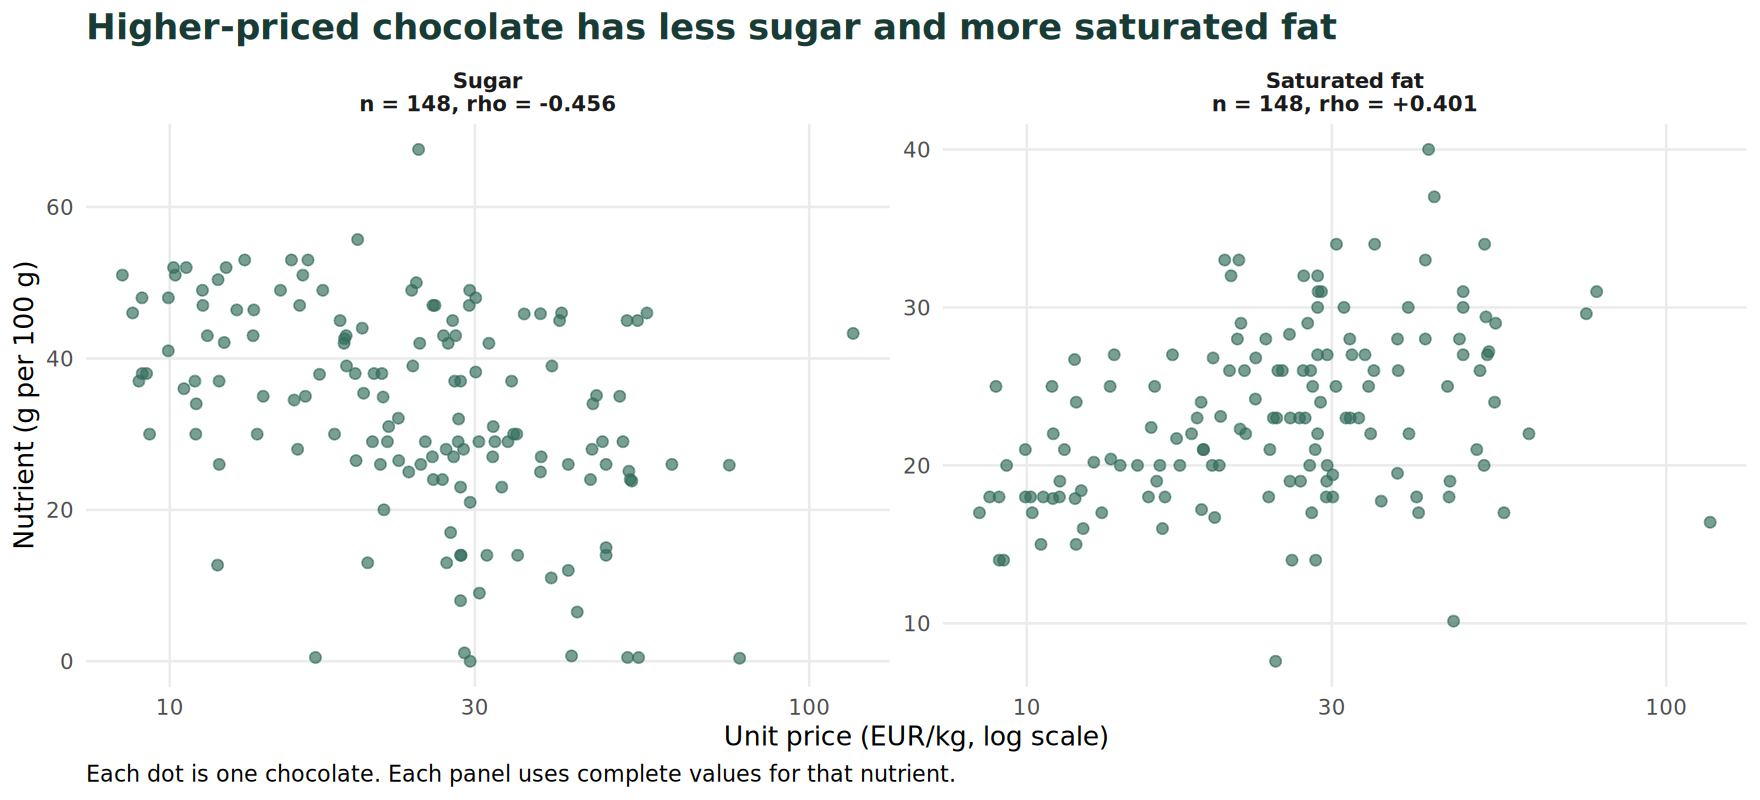
\includegraphics[width=\linewidth,height=.30\textheight,keepaspectratio]{generated/figures/en/chocolate_composition.png}\caption{Two chocolate nutrients move in opposite directions with price. The horizontal axis shows logarithmic unit price and the vertical axis shows grams per 100 g. Each dot is a product. Sugar has a negative price association in the left panel and saturated fat a positive association in the right panel.}\label{fig:composition}\end{figure}

\subsection{Most jointly observed products have a lower-price candidate}
Of 583 products with all three measures, 562 (96.4\%) have at least one lower-priced same-category candidate with neither grade worse. Category shares range from 95.2\% to 98.6\% (Table~\ref{tab:candidates}). This answers RQ3 and identifies individual comparisons beyond the overall price--score patterns.
\begin{table}[!ht]\centering\small\caption{Products with a lower-price candidate. Each product is counted once if at least one other product meets both grade conditions.}\begin{tabular}{lrrrr}
\toprule
Category & Joint $n$ & With candidate & Share & Non-dominated \\
\midrule
Biscuits & 146 & 139 & 95.2\% & 7 \\
Breakfast cereals & 147 & 145 & 98.6\% & 2 \\
Dark chocolate & 146 & 139 & 95.2\% & 7 \\
Fruit juices & 144 & 139 & 96.5\% & 5 \\
\bottomrule
\end{tabular}
\label{tab:candidates}\end{table}

\begin{table}[!ht]\centering\small\caption{An illustrative biscuit pair. B has a 45.7\% lower historical unit price, the same nutrition grade and a better environmental grade.}\begin{tabular}{lrr}
\toprule
Measure & Product A & Candidate B \\
\midrule
Barcode & 3350031923081 & 3410280136257 \\
Unit price (EUR/kg) & 7.36 & 4.00 \\
Nutrition grade & E & E \\
Environmental grade & C & B \\
\bottomrule
\end{tabular}
\label{tab:pair}\end{table}
In Table~\ref{tab:pair}, A is Galettes bretonnes pur beurre and B is Petit beurre 200g. Their representative prices are EUR 7.36/kg and EUR 4.00/kg, a difference of EUR 3.36/kg. Both have nutrition grade E, while their environmental grades are C and B. A has two regular offers, and B's single offer dates from 10 January 2024. These attributes make B a candidate for checking recipe, pack suitability and current store price.

\subsection{Price definitions and offer coverage affect interpretation}
Including discounted offers changes 15 representative prices, and retaining duplicate observations also changes 15. Among products with multiple regular offers, cereals and chocolate retain the original directions for both composite scores, while biscuits and juices remain close to zero. For the same juice products, changing from price per litre to price per 100 kcal changes the nutrition correlation from $0.041$ to $-0.153$. Volume and energy units answer different comparison questions. The main analysis uses kg/L to match retail quantities.

\section{Discussion}
Together, the results support category-specific product comparison. Prices carry some nutrition and environmental score information for cereals and dark chocolate, while biscuits and juices call for direct inspection of attributes. Chocolate shows how a favourable direction in a composite score can coexist with a nutrient trade-off. The lower-price analysis brings these patterns into a two-product comparison that readers can assess against their intended use.

The findings align with previous attention to food-group differences and functional units\cite{masset2015,martinez2025}. The eight-source review also provides context on sustainable foods, price trends and green premiums\cite{masset2014,hoenink2024,nakavachara2025,clark2022,desiderio2026,bai2025}. This project illustrates those differences in four packaged-food categories and makes the comparisons available for interactive inspection.

The contribution-based price records and balanced category sample describe the products observed in this study. One regular offer supports 291 products, and historical prices precede the 2026 product snapshot. Coarse grades increase the chance that products share a grade, while taste and intended use affect substitution. AGRIBALYSE 3.2 carbon estimates cover 594 products, but the 150 cereals share only four distinct carbon values through reference-food mappings. These features define the scope of the comparison. Current store prices and more detailed recipe and use groups would extend it.

\section{Shiny Dashboard}
The dashboard follows the three research questions. The overview shows the category price distribution and reports nutrition and environmental relationships separately. Explore places the question, axis definitions and current finding beside the same chart. Filtering recalculates both the association and its available sample. Chocolate users can switch between sugar and saturated fat, then examine two products with their price and composition differences.

Consumers can set a category budget and inspect suitable alternatives. Suppliers or product analysts can use the same findings to benchmark retail positioning and attributes. The role changes the suggested action. Classroom trials can record completion and time for a product-selection task and assess whether users can explain their choice. Further commercial analysis would add current prices, internal costs and customer evidence.

\section{Conclusion}
Across these four French packaged-food categories, the relationship between price, nutrition and environmental performance varies by category. Higher-priced cereals and chocolate tend to have better composite scores, while biscuit and juice associations are close to zero. Chocolate combines lower sugar with higher saturated fat as price increases, making composition central to the comparison. Among 583 jointly observed products, 562 have a cheaper same-category candidate with neither grade worse.

\textbf{Our interpretation is to use unit price to set a budget, then compare grades and composition at product level.} The Shiny workflow implements that sequence through category selection, chart exploration and two-product comparison. It helps readers explain which attributes accompany a higher price and whether a lower-price candidate fits their purpose.

\appendix
\section{Reproduction, sources and assistance}
Analysis code is in \nolinkurl{R/10_eda.R} and the full notebook in \nolinkurl{notebooks/step4_eda.Rmd}. Four numerical tables are generated from \nolinkurl{outputs/step4/tables/}. Report exhibits are drawn by \nolinkurl{scripts/build_report_figures.R}, with shared data and plotting rules for both languages. Run \nolinkurl{scripts/run_step4.ps1} to reconstruct the analysis, \nolinkurl{scripts/build_report.ps1} to compile the reports and \nolinkurl{scripts/run_shiny.ps1} to start the application.

Data are credited to Open Prices / Open Food Facts contributors, with licences and processing records in \nolinkurl{data/README.md}. The report uses Tau-class 2.6.0 by Guillermo Jimenez, CC BY 4.0. Dashboard context imagery is AI-generated, with provenance in \nolinkurl{reports/assets/provenance.json}. AI assisted with code generation, report drafting and checks. Named member contributions, individual reflections and classroom feedback will be supplied by the group for course submission. Review summaries for Masset (2014) and Bai (2025) are based on abstracts, with reading coverage recorded in the literature review.
\begin{thebibliography}{9}\small
\bibitem{masset2014} Masset, G., et al. (2014). Identifying sustainable foods: The relationship between environmental impact, nutritional quality, and prices of foods representative of the French diet. \textit{JAND, 114}, 862--869. \url{https://doi.org/10.1016/j.jand.2014.02.002}.
\bibitem{masset2015} Masset, G., Vieux, F., \& Darmon, N. (2015). Which functional unit to identify sustainable foods? \textit{Public Health Nutrition, 18}, 2488--2497. \url{https://doi.org/10.1017/S1368980015000579}.
\bibitem{hoenink2024} Hoenink, J. C., et al. (2024). Changes in UK price disparities between healthy and less healthy foods over 10 years. \textit{Appetite, 197}, 107290. \url{https://doi.org/10.1016/j.appet.2024.107290}.
\bibitem{martinez2025} Martinez, E. M., et al. (2025). Retail prices, environmental footprints, and nutritional profiles of commonly sold retail food items in 181 countries. \textit{AJCN, 122}, 1265--1274. \url{https://doi.org/10.1016/j.ajcnut.2025.08.002}.
\bibitem{nakavachara2025} Nakavachara, V., et al. (2025). The green premium puzzle. Preprint, v1. \url{https://arxiv.org/abs/2507.10333v1}.
\bibitem{clark2022} Clark, M., et al. (2022). Estimating the environmental impacts of 57,000 food products. \textit{PNAS, 119}, e2120584119. \url{https://doi.org/10.1073/pnas.2120584119}.
\bibitem{desiderio2026} Desiderio, A., et al. (2026). Mapping regional disparities in discounted grocery products. \textit{npj Science of Food, 10}, 112. \url{https://doi.org/10.1038/s41538-026-00764-0}.
\bibitem{bai2025} Bai, Y., et al. (2025). Environmental impacts and monetary costs of healthy diets worldwide. \textit{Nature Food, 6}, 1176--1185. \url{https://doi.org/10.1038/s43016-025-01270-4}.
\end{thebibliography}
\end{document}
